\documentclass[a4paper,12pt]{report}
\usepackage[utf8]{inputenc}
\usepackage{amsmath}
\usepackage{graphicx}
\usepackage{listings}
\usepackage{tikz}
\usepackage[T1]{fontenc}
\usepackage{color}
\usetikzlibrary{arrows,automata}
\definecolor{pythonred}{rgb}{0.6,0,0} % for strings
\definecolor{pythongreen}{rgb}{0.25,0.5,0.35} % comments
\definecolor{pythonpurple}{rgb}{0.5,0,0.35} % keywords
	\definecolor{pythondocblue}{rgb}{0.25,0.35,0.75} % javadoc
	 
	\lstset{language=python,
	basicstyle=\ttfamily,
	keywordstyle=\color{pythonpurple}\bfseries,
	stringstyle=\color{pythonred},
	commentstyle=\color{pythongreen},
	morecomment=[s][\color{pythondocblue}]{/**}{*/},
	numbers=left,
	numberstyle=\tiny\color{black},
        stepnumber=2,
	numbersep=10pt,
	tabsize=4,
	showspaces=false,
	showstringspaces=false}

% Title Page

 \title{\bfseries\huge \textcolor{purple}{\underline {EEP702-Software Lab}} \\{\textcolor{blue}{Assignment 8 : Basics of Designing Applicaton in Qt}}}
\author{\bfseries\large\textcolor{black}  {Harshit Kumar Gupta}\\ {\textcolor{black} {2013EET2369 }}\\

\includegraphics[width=3cm,height=3.4cm]{iit.png}\\\noindent Computer Technology\\
\noindent Department Of Electrical Engineering\\IIT DELHI}
% iit.png: 282x282 pixel, 72dpi, 9.95x9.95 cm, bb=0 0 282 282
\begin{document}
\maketitle
\tableofcontents


\chapter{\textcolor{blue}{\underline {PROBLEM STATEMENT}}}
\noindent Develop a Library Management System:
\begin{enumerate}
\item Design a user interface(GUI) in Qt.The user will be asked to enter a number in numeric (say, 55) and will be provided a button named “Convert to text”.On pressing this button, the entered number should be displayed in words (fifty five).
\item Add one more feature to the above GUI, which will enable user to enter a number in text (fifty five). Add one button named “Convert  to Number”, on pressing which the entered number in words will be shown in numeric digits (55).
\item Add one more feature to the above GUI, which will enable user to enter a number in text (fifty five) and display a comma separated value as it is typed in (note that the internal representation will be without commas of course).
\end{enumerate}

\noindent Use Qt to design the Application.\\\\


\begin{center}
\chapter{\textcolor{blue}{\underline {ABSTRACT}}}
\end{center}
\noindent The intention is to learn designing in Qt.

\begin{enumerate}
\item Qt is a cross-platform application framework that is widely used for developing application software with a graphical user interface (GUI) (in which cases Qt is classified as a widget toolkit), and also used for developing non-GUI programs such as command-line tools and consoles for servers.
\item Qt uses standard C++ but makes extensive use of a special code generator (called the Meta Object Compiler, or moc) together with several macros to enrich the language. Qt can also be used in several other programming languages via language bindings. It runs on the major desktop platforms and some of the mobile platforms. It has extensive internationalization support. Non-GUI features include SQL database access, XML parsing, thread management, network support, and a unified cross-platform application programming interface (API) for file handling.
\end{enumerate}

\begin{center}
\chapter{\textcolor{blue}{\underline {INTRODUCTION}}}
\end{center}

\noindent Qt, when it was first released, relied on a few key concepts:
\begin{enumerate}
\item 
    Complete abstraction of the GUI – When first released, Qt used its own paint engine and controls, emulating the look of the different platforms it runs on when it drew its widgets. This made the porting work easier because very few classes in Qt depended really on the target platform; however, this occasionally led to slight discrepancies where that emulation was imperfect.

    Recent versions of Qt use the native style APIs of the different platforms, on platforms that have a native widget set, to query metrics and draw most controls, and do not suffer from such issues as much.[53]

    On some platforms (such as MeeGo and KDE) Qt is the native API.

    Some other portable graphical toolkits have made different design decisions; for example, wxWidgets uses the toolkits of the target platform for its implementations.
\item Signals and slots - a language construct introduced in Qt for communication between objects[54] which makes it easy to implement the Observer pattern while avoiding boilerplate code. The concept is that GUI widgets can send signals containing event information which can be received by other controls using special functions known as slots.
\item Metaobject compiler - The metaobject compiler, termed moc, is a tool that is run on the sources of a Qt program. It interprets certain macros from the C++ code as annotations, and uses them to generate added C++ code with Meta Information about the classes used in the program. This meta information is used by Qt to provide programming features not available natively in C++: signals and slots, introspection and asynchronous function calls.
\end{enumerate}

\begin{center}
\chapter{\textcolor{blue}{\underline {SPECIFICATIONS AND ASSUMPTIONS}}}

\section*{Specifications}

\begin{enumerate}
\item Design a user interface(GUI) in Qt.
\item User should be asked to enter either number or text to convert it to text and numbers correspondingly.
\item Converted number should be formated in indian number format Ex: 11,12,256.
\end{enumerate}

\section*{Assumptions}

\begin{enumerate}
\item If user enters wrong number output displays as zero.
\item If user enters wrong text output displays as 0.
\item If user entered number is negative or out of range, output displays as unsupported.
\end{enumerate}
 
\begin{center}
\chapter{\textcolor{blue}{\underline {LOGIC USED/METHODOLOGY}}}
\end{center}
The methodology that is used for developing the program is defined below:\\
\begin{center}
\begin{enumerate}
\item Storing all strings for digits in arrays.
\item Deviding the number with corresponding weight and concating to global variable result the words according to digits and weight.
\item Implemented above functionality in a function and calling the function when user clicks the button.
\item Text to numbers implemented using python and calling the python script from Qt using QtProcess.
\item Formating the number into indian number format using string stream.
\end{enumerate}
\end{center}

\begin{center}
\chapter{\textcolor{blue}{\underline {FLOWCHART}}}

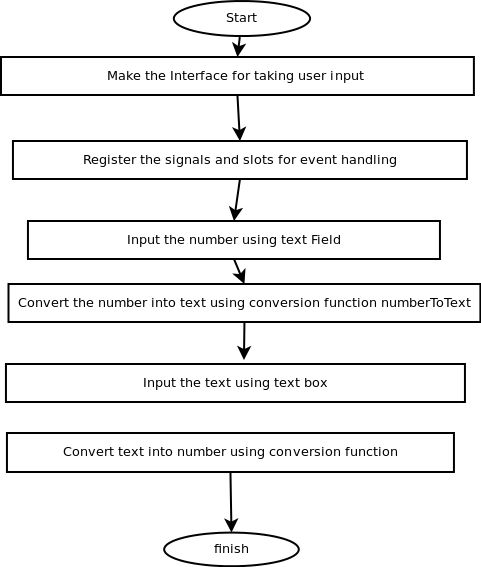
\includegraphics[width=13 cm,height=12 cm]{flowchart.png}
\end{center}



\begin{center}

\chapter{\textcolor{blue}{\underline {RESULTS AND CONCLUSIONS}}}\end{center}
\begin{center}
\begin{enumerate}
\item Could convert number to text.
\item Could convert text to number.
\item Could format number to indian number format.
\item We can use espeak command and QtProcess type to produce voice for given text.
\begin{center}
\chapter{\textcolor{blue}{\underline {OUTPUTS OF PROGRAM}}}
\end{center}
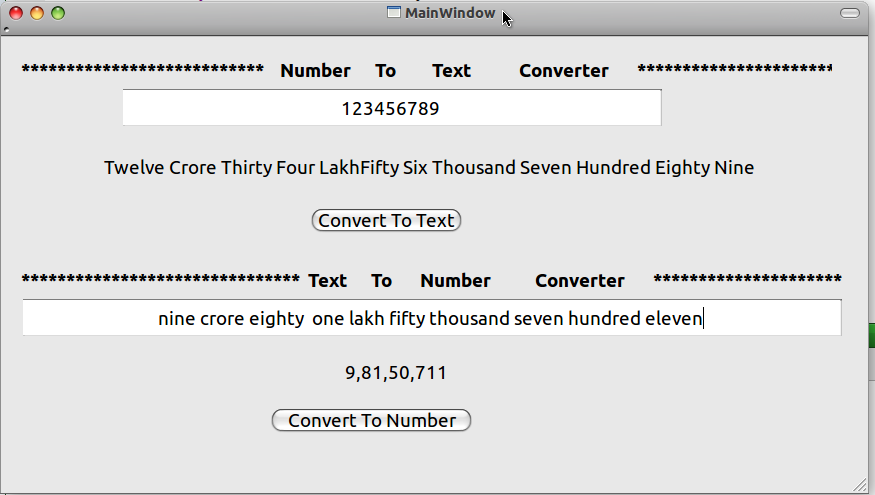
\includegraphics[width=13 cm,height=12 cm]{Screenshot-1.png}
\\[1 cm] Figure 2: Application GUI Screen with Results .\\
\end{enumerate}
\end{center}

\end{document}  
